\documentclass[12pt]{../../oss-apphys-exam}
\usepackage{enumitem}

\usetikzlibrary{patterns}

\tikzset{
  >=latex
}

\runningheader{
  \fontfamily{phv}\small
  \textcolor{gray}{AP PHYSICS C: MECHANICS $\blacksquare$}
  \textbf{MULTIPLE-CHOICE QUESTIONS}}{}{}


\begin{document}

\begin{center}
  {
    \fontfamily{phv}\Large
    \textbf{AP PHYSICS C: MECHANICS\\SECTION I\\TIME -- 55 MINUTES}
  }
\end{center}

\textbf{Directions:} Each of the questions or incomplete statements below is
followed by five suggested answers or completions. Select the one that is best
in each case and place the letter of your choice in the corresponding box on
the student answer sheet.

\vspace{.2in}\textbf{Note:} To simplify calculations, you may use
$g=\SI{10}{\metre\per\second\squared}$ in all problems.

\begin{questions}

  \question A sphere of mass $m$ is dropped from the top of a building and
  reaches the ground before achieving terminal velocity. The force of air
  resistance that acts on the sphere as it falls is given by $F=-kv$, where
  $k$ is a positive constant and $v$ is the velocity of the sphere. What
  happens to the magnitude of the sphere's velocity and acceleration, and to
  the distance it falls during each second, as the sphere approaches the ground?
  
  \begin{tabular}{cccc}
    & \textbf{Magnitude of Velocity}
    & \textbf{Magnitude of Acceleration}
    & \textbf{Distance of Fall Each Second}\\ \hline
    (A) & Increases & Increases & Increases\\
    (B) & Increases & Decreases & Increases\\
    (C) & Increases & Decreases & Decreases\\
    (D) & Decreases & Increases & Decreases\\
    (E) & Decreases & Decreases & Increases
  \end{tabular}
  \newpage
  
  \question The net force $F$ acting on an object that moves along a straight
  line is given as a function of time $t$ by $F(t)=\kappa t^2 +\tau$ , where
  $\kappa=\SI1{\newton\per\second\squared}$ and $\tau =\SI1\newton$. What is
  the change in momentum of the object from $t=\SI0\second$ to $t=\SI3\second$?
  \begin{choices}
    \choice\SI6{\kilo\gram\metre\per\second}
    \choice\SI{10}{\kilo\gram\metre\per\second}
    \choice\SI{12}{\kilo\gram\metre\per\second}
    \choice\SI{30}{\kilo\gram\metre\per\second}
    \choice It cannot be determined without knowing the initial momentum of the
    object.
  \end{choices}
  \newpage
  
  \question A ball of mass $m$ is dropped from rest at a height $h$ and collides
  elastically with the floor, rebounding to its original height. What is the
  magnitude of the net impulse on the ball during the collision with the floor?
  \begin{choices}
    \choice Zero
    \choice $m\sqrt{gh}$
    \choice $m\sqrt{2gh}$
    \choice $2m\sqrt{gh}$
    \choice $2m\sqrt{2gh}$
  \end{choices}
  \newpage
  
  \question A student initially stands on a circular platform that is free to
  rotate without friction about its centre. The student jumps off tangentially,
  setting the platform spinning. Quantities that are conserved for the
  student-platform system as the student jumps include which of the following?
  \begin{enumerate}[nosep]
  \item[I.] Angular momentum
  \item[II.] Linear momentum
  \item[III.] Kinetic energy
  \end{enumerate}  
  \begin{choices}
    \choice I only
    \choice II only
    \choice I and II only
    \choice II and III only
    \choice I, II, and III
  \end{choices}
  \newpage
  
  % THIS QUESTION IS TAKEN FROM THE 2019 AP PHYSICS C MECHANICS SAMPLE TEST
  % MULTIPLE-CHOICE QUESTION #24
  \uplevel{
    \cpic{.32}{2disks}
  }
  \question Two horizontal disks of mass $M$ have the radii shown above. Disk
  $A$ is attached to an axle of negligible mass spinning freely with angular
  velocity $\omega_0$. Disk $B$, not attached to the axle and initially held
  at rest, is released and drops down onto disk $A$. When both disks spin
  together without slipping, the angular velocity $\omega_f$ of the disks is
  \begin{choices}
    \choice $\dfrac13\omega_0$
    \choice $\dfrac12\omega_0$
    \choice $\dfrac23\omega_0$
    \choice $\dfrac45\omega_0$
    \choice $\dfrac2{\sqrt5}\omega_0$
  \end{choices}
  \newpage
  
  \uplevel{
    \textbf{Questions \ref{beam1}--\ref{beam2}}
    
    \vspace{-.2in}
    \cpic{.3}{beam}

    \vspace{-.2in}The bar shown above is pivoted about one end and is initially
    at rest in a vertical position. The bar is displaced slightly and as it
    falls it makes an angle $\theta$ with the vertical at any given time, as
    shown above.
  }
  \question Which of the following graphs best represents the bar's angular
  acceleration $\alpha$ as a function of angle $\theta$?

  \begin{oneparchoices}
    \choice
    \begin{tikzpicture}[scale=1.2]
      \draw[axes] (0,0)--(2,0) node[right]{$\theta$};
      \draw[axes] (0,0)--(0,2) node[above]{$\alpha$};
      \draw[ultra thick] (0,1)--(1.8,1);
    \end{tikzpicture}

    \choice
    \begin{tikzpicture}[scale=1.2]
      \draw[axes] (0,0)--(2,0) node[right]{$\theta$};
      \draw[axes] (0,0)--(0,2) node[above]{$\alpha$};
      \draw[ultra thick] (0,0)--(1.6,1.6);
    \end{tikzpicture}

    \choice
    \begin{tikzpicture}[scale=1.2]
      \draw[axes] (0,0)--(2,0) node[right]{$\theta$};
      \draw[axes] (0,0)--(0,2) node[above]{$\alpha$};
      \draw[ultra thick] (0,1.5)--(1.6,0);
    \end{tikzpicture}

    \choice
    \begin{tikzpicture}[scale=1.2]
      \draw[axes] (0,0)--(2,0) node[right]{$\theta$};
      \draw[axes] (0,0)--(0,2) node[above]{$\alpha$};
      \draw[ultra thick,domain=0:1.8] plot(\x,{1.5*sin(48*\x)});
    \end{tikzpicture}

    \choice
    \begin{tikzpicture}[scale=1.2]
      \draw[axes] (0,0)--(2,0) node[right]{$\theta$};
      \draw[axes] (0,0)--(0,2) node[above]{$\alpha$};
      \draw[ultra thick,domain=0:1.8] plot(\x,{-1.5*cos(48*\x)+1.5});
    \end{tikzpicture}
  \end{oneparchoices}
  \label{beam1}
  
  \question Which of the following graphs best represents the bar's angular
  velocity $\omega$ as a function of time?

  \begin{oneparchoices}
    \choice
    \begin{tikzpicture}[scale=1.2]
      \draw[axes] (0,0)--(2,0) node[right]{$t$};
      \draw[axes] (0,0)--(0,2) node[above]{$\omega$};
      \draw[ultra thick] (0,1)--(1.8,1);
    \end{tikzpicture}

    \choice
    \begin{tikzpicture}[scale=1.2]
      \draw[axes] (0,0)--(2,0) node[right]{$t$};
      \draw[axes] (0,0)--(0,2) node[above]{$\omega$};
      \draw[ultra thick] (0,1.6)--(1.6,0);
    \end{tikzpicture}

    \choice
    \begin{tikzpicture}[scale=1.2]
      \draw[axes] (0,0)--(2,0) node[right]{$t$};
      \draw[axes] (0,0)--(0,2) node[above]{$\omega$};
      \draw[ultra thick,domain=0:1.8] plot(\x,{1.5*sin(48*\x)});
    \end{tikzpicture}

    \choice
    \begin{tikzpicture}[scale=1.2]
      \draw[axes] (0,0)--(2,0) node[right]{$t$};
      \draw[axes] (0,0)--(0,2) node[above]{$\omega$};
      \draw[ultra thick,domain=0:1.6] plot(\x,{1.5*cos(56*\x)});
    \end{tikzpicture}

    \choice
    \begin{tikzpicture}[scale=1.2]
      \draw[axes] (0,0)--(2,0) node[right]{$t$};
      \draw[axes] (0,0)--(0,2) node[above]{$\omega$};
      \draw[ultra thick,domain=0:1.8] plot(\x,{-1.5*cos(48*\x)+1.5});
    \end{tikzpicture}
  \end{oneparchoices}
  \label{beam2}
  \newpage
  
  \uplevel{
    \centering
    \begin{tikzpicture}[scale=1.2,thick]
      \draw (0,0)--(2,0);
      \draw (2,0) rectangle (3,3);
      \fill (1,1) circle (.07) node[left]{$P$};
      \draw[fill=gray!70] (1.7,2.5) circle (.11);
      \draw[vectors] (1.7,2.3)--(1.7,1.5);
    \end{tikzpicture}
  }
  
  \question A stone falls from rest from the top of a building as shown above.
  Which of the following graphs best represents the stone's angular momentum $L$
  about the point $P$ as a function of time?

  \begin{oneparchoices}
    \choice
    \begin{tikzpicture}[scale=1.2]
      \draw[axes] (0,0)--(2,0) node[right]{$t$};
      \draw[axes] (0,0)--(0,2) node[above]{$L$};
      \draw[ultra thick] (0,0)--(1.8,0);
    \end{tikzpicture}

    \choice
    \begin{tikzpicture}[scale=1.2]
      \draw[axes] (0,0)--(2,0) node[right]{$t$};
      \draw[axes] (0,0)--(0,2) node[above]{$L$};
      \draw[ultra thick] (0,1.2)--(1.6,1.2);
    \end{tikzpicture}

    \choice
    \begin{tikzpicture}[scale=1.2]
      \draw[axes] (0,0)--(2,0) node[right]{$t$};
      \draw[axes] (0,0)--(0,2) node[above]{$L$};
      \draw[ultra thick] (0,0)--(1.6,1.5);
    \end{tikzpicture}

    \choice
    \begin{tikzpicture}[scale=1.2]
      \draw[axes] (0,0)--(2,0) node[right]{$t$};
      \draw[axes] (0,0)--(0,2) node[above]{$L$};
      \draw[ultra thick,domain=0:1.6] plot(\x,{-1.5*cos(56*\x)+1.5});
    \end{tikzpicture}
    
    \choice
    \begin{tikzpicture}[scale=1.2]
      \draw[axes] (0,0)--(2,0) node[right]{$t$};
      \draw[axes] (0,0)--(0,2) node[above]{$L$};
      \draw[ultra thick,domain=0:1.8] plot(\x,{1.5*sin(100*\x)});
    \end{tikzpicture}
  \end{oneparchoices}
  \newpage
  
  \uplevel{
    \textbf{Questions \ref{ladder1}--\ref{ladder2} refer to the following
      diagram:}
    \begin{center}
      \begin{tikzpicture}[thick,scale=.85]
        \draw (0,5)--(0,0) node[pos=0,above]{Wall}--(4,0) node[above]{Floor};
        \begin{scope}[rotate around = {atan(.75):(3,0)}]
          \draw[fill=gray] (3,0) rectangle (3.2,5)
          node[midway,above right]{Ladder};
        \end{scope}
        \draw[axes] (1.5,0) arc (180:180-atan(4/3):1.5)
        node[midway,left=-1]{$\theta$};
      \end{tikzpicture}
    \end{center}
    A uniform ladder of weight $W$ leans without slipping against a wall making
    an angle $\theta$ with a floor as shown above. There is friction between
    the ladder and the floor, but the friction between the ladder and the wall
    is negligible.
  }

  \question The magnitude of the normal force exerted by the floor on the ladder
  is  
  \begin{choices}
    \choice $W$
    \choice $W\sin\theta$
    \choice $W\cos\theta$
    \choice $\dfrac W2\sin\theta$
    \choice $\dfrac W2\cos\theta$
  \end{choices}
  \label{ladder1}
  
  \question The magnitude of the friction force exerted on the ladder by the
  floor is  
  \begin{choices}
    \choice $2W\tan\theta$
    \choice $W$
    \choice $W\cot\theta$
    \choice $\dfrac W2$
    \choice $\dfrac W2\cot\theta$
  \end{choices}
  \label{ladder2}
  \newpage
  
  % THIS QUESTION IS TAKEN FROM THE 2019 PRACTICE TEST QUESTIONS 23
  \uplevel{
    \centering
    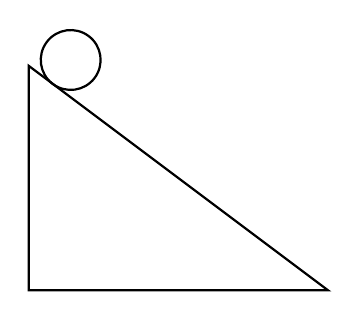
\begin{tikzpicture}[thick,scale=.95]
      \draw (0,0)--(0,-3)--(4,-3)--cycle;
      \draw[rotate=-37] (.4,.4) circle (.4);
    \end{tikzpicture}
  }
  
  \question A sphere starts from rest at the top of a ramp, as shown above. It
  rolls without slipping down the ramp. The potential energy of the sphere-Earth
  system is zero at the bottom of the ramp. Which of the following is true of
  the sphere when it reaches the bottom of the ramp?
  \begin{choices}
    \choice Its rotational kinetic energy equals the initial potential energy
    of the sphere-Earth system.
    \choice Its translational kinetic energy equals the initial potential
    energy of the sphere-Earth system.
    \choice Its translational kinetic energy and rotational kinetic energy are
    equal.
    \choice The sum of its translational kinetic energy and rotational kinetic
    energy equals the initial potential energy of the sphere-Earth system.
    \choice The sum of its translational kinetic energy and rotational kinetic
    energy equals the energy lost because of friction
  \end{choices}
  \newpage
  
  % THESE QUESTIONS ARE TAKEN FROM THE 2019 PRACTICE TEST QUESTIONS 4-6
  \uplevel{
    \textbf{Questions \ref{car1}--\ref{car3}}
    \begin{center}
      \pic{.3}{car-turning}\\
      \underline{Note:} Figure not drawn to scale.
    \end{center}
    A car is travelling clockwise around a circular racetrack of radius
    \SI{1440}\metre. When the car is at the northernmost point on the circle,
    as shown above, it has a speed of \SI{36.0}{\metre\per\second} and is
    slowing down at a rate of \SI{1.20}{\metre\per\second\squared}.
  }

  \question The direction of the velocity of the car is
  \label{car1}
  \begin{choices}
    \choice due east
    \choice south of east
    \choice due south
    \choice south of west
    \choice due west
  \end{choices}

  \question The direction of the acceleration of the car is
  \begin{choices}
    \choice due east
    \choice south of east
    \choice due south
    \choice south of west
    \choice due west
  \end{choices}
  
  \question What is the magnitude of the acceleration of the car?
  \label{car3}
  \begin{choices}
    \choice $\SI{.30}{\metre\per\second\squared}$
    \choice $\SI{.90}{\metre\per\second\squared}$
    \choice $\SI{1.2}{\metre\per\second\squared}$
    \choice $\SI{1.5}{\metre\per\second\squared}$
    \choice $\SI{2.1}{\metre\per\second\squared}$
  \end{choices}
  \newpage
  
  \question An ideal spring with spring constant $k$ is cut in half. What is the
  spring constant of either one of the two half springs?
  \begin{choices}
    \choice $\dfrac k2$
    \choice $\sqrt k$
    \choice $k$
    \choice $k^2$
    \choice $2k$
  \end{choices}
  \newpage
  
  \question An object on the end of a spring with spring constant $k$ moves in
  simple harmonic motion with amplitude $A$ and frequency $f$. Which of the
  following is a possible expression for the kinetic energy of the object as a
  function of time $t$?
  \begin{choices}
    \choice $kA^2 \sin^2(2\pi ft)$
    \choice $\dfrac12kA^2\cos^2(2\pi ft)$
    \choice $\dfrac12kA\sin(2\pi ft)$
    \choice $kA\cos(2\pi ft)$
    \choice $kA\left(\sin(2\pi ft)+\cos(2\pi ft)\right)$
  \end{choices}
  \newpage
  
  % THE NEXT 3 QUESTIONS ARE TAKEN FROM THE 2019 PRACTICE TEST QUESTIONS 32-34
  \uplevel{
    \textbf{Questions \ref{spring1}--\ref{spring2}}
    \begin{center}
      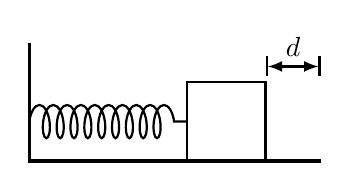
\begin{tikzpicture}[thick]
        \draw (2,0) rectangle +(1,1);
        \draw[decoration={aspect=.4,segment length=5,amplitude=6,coil},
          decorate] (0,.5)--(2,.5);
        \draw[very thick] (0,1.5)--(0,0)--(3.7,0);
        \draw[|<->|] (3,1.2)--+(.7,0) node[midway,above]{$d$};
      \end{tikzpicture}
      \hspace{.5in}
      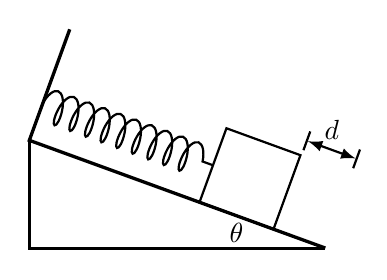
\begin{tikzpicture}[thick]
        \begin{scope}[rotate=-20]
          \draw (2.3,0) rectangle +(1,1);
          \draw[decoration={aspect=.37,segment length=6,amplitude=6,coil},
            decorate] (0,.5)--+(2.3,0);
          \draw[very thick] (0,1.5)--(0,0)--(4,0);
          \draw[|<->|] (3.3,1.2)--+(.7,0) node[midway,above]{$d$};
        \end{scope}
        \draw[very thick] (0,0)--(0,-1.37)
        --(3.76,-1.37) node[pos=.7,above=-2]{$\theta$};
      \end{tikzpicture}
    \end{center}
    Systems A and B contain identical ideal springs and identical blocks that
    can slide along a surface of negligible friction. In system A, the surface
    is horizontal. In system B, the surface makes an angle $\theta$ with the
    horizontal. Initially, both blocks are at rest and in equilibrium. Each
    block is then pulled the same distance $d$ in the direction shown in the
    figures and released from rest at $t=0$.
  }
  \question After the block in system A is released from rest, the time for the
  block to first reach a maximum speed is $\Delta t_A$. After the block in
  system B is released, the time for the block to first reach a maximum speed is
  \label{spring1}
  \begin{choices}
    \choice $\Delta t_A$
    \choice $\Delta t_A\sin\theta$
    \choice $\dfrac{\Delta t_A}{\sin\theta}$
    \choice $\Delta t_A\cos\theta$
    \choice $\dfrac{\Delta t_A}{\cos\theta}$
  \end{choices}
  
  \question For system A, when the block is halfway between its release
  position and its equilibrium position, the block's kinetic energy is $K$ and
  the elastic potential energy of the spring-block system is $U$. The ratio
  $K/U$ is
  \begin{choices}
    \choice $1/3$
    \choice $1/2$
    \choice $1/1$
    \choice $2/1$
    \choice $3/1$
  \end{choices}
  \question A student wants to use an apparatus similar to system B to measure
  the acceleration due to gravity $g$. If the mass of the block, the force
  constant of the spring, and the angle of the incline are known, what
  additional data must be measured to determine an experimental value for $g$?
  \label{spring2}
  \begin{itemize}[nosep]
    \item[I.] The stretch of the spring at the equilibrium position
    \item[II.] The speed of the block as it passes the equilibrium position
    \item[III.] The time interval between two consecutive passes through the
      equilibrium position
  \end{itemize}
  \begin{choices}
    \choice I only
    \choice II only
    \choice I and II
    \choice II and III
    \choice I and III
  \end{choices}
  \newpage
  
  \question In an experiment with a simple pendulum, measurements of the period
  $T$ of the pendulum are made for different values of its length $L$.
  When plotted on a graph, which of the following should result in a
  straight-line fit of the data?
  \begin{choices}
    \choice $\sqrt T$ versus $L$
    \choice $T$ versus $L$
    \choice $T$ versus $L^2$
    \choice $T^2$ versus $L$
    \choice $T^2$ versus $L^2$
  \end{choices}
  \newpage
  
  % THIS QUESTION IS TAKEN FROM THE 2019 PRACTICE TEST QUESTIONS 31
  \uplevel{
    \centering
    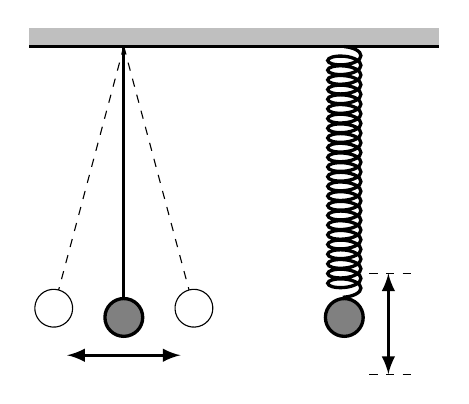
\begin{tikzpicture}[scale=.8]
      \fill[lightgray] rectangle (6.5,.3);
      \draw[very thick] (0,0)--(6.5,0);
      \draw[very thick] (1.5,0)--+(0,-4);
      \draw[very thick,fill=gray] (1.5,-4.3) circle (.3);
      \begin{scope}[rotate around={15:(1.5,0)}]
        \draw[dashed] (1.5,0)--+(0,-4);
        \draw (1.5,-4.3) circle (.3);
      \end{scope}
      \begin{scope}[rotate around={-15:(1.5,0)}]
        \draw[dashed] (1.5,0)--+(0,-4);
        \draw (1.5,-4.3) circle (.3);
      \end{scope}
      \draw[very thick,<->] (.6,-4.9)--(2.4,-4.9);
      \draw[very thick,
        decoration={aspect=.4,segment length=3.5,amplitude=6,coil},
        decorate] (5,0)--+(0,-4);
      \draw[very thick,fill=gray] (5,-4.3) circle (.3);
      \draw[very thick,<->] (5.7,-3.6)--(5.7,-5.2);
      \foreach \y in {-3.6,-5.2} \draw[dashed] (5.4,\y)--+(.7,0);
    \end{tikzpicture}
  }
  \question A pendulum and a spring both have a \SI1{\kilo\gram} sphere
  attached to their ends and have the same length when in equilibrium, as shown
  in the figure above. They both oscillate with the same period. If the
  \SI1{\kilo\gram} spheres are replaced with \SI2{\kilo\gram} spheres and the
  amplitudes of oscillation are unchanged, which of the following is true about
  the resultant period of oscillation for each?
  
  \begin{tabular}{cll}
    & \textbf{Pendulum} & \textbf{Spring} \\ \hline
    (A) & Remains the same\hspace{.3in} & Decreases\\
    (B) & Remains the same & Increases\\
    (C) & Remains the same & Remains the same\\
    (D) & Increases        & Remains the same\\
    (E) & Increases        & Increases
  \end{tabular}
  \newpage
  
  \cpic{.15}{comet}
  \question A comet moves in the Sun's gravitational field, following the path
  shown above. What happens to its angular momentum as it moves from point $X$
  to point $Y$?
  \begin{choices}
    \choice It increases steadily.
    \choice It remains constant.
    \choice It decreases steadily.
    \choice It increases as it approaches the Sun and decreases as it moves
    away from the Sun.
    \choice It decreases as it approaches the Sun and increases as it moves
    away from the Sun.
  \end{choices}
  \newpage
  
  \uplevel{
    \textbf{Questions \ref{orbit1}--\ref{orbit2}}
    \begin{center}
      \pic{.38}{orbit}\\
      \underline{Note:} Figure not drawn to scale.
    \end{center}
    A moon of mass $m$ orbits a planet of mass $49m$ in an elliptical orbit as
    shown above. When the moon is at point $A$, its distance from the centre of
    the planet is $r_A$ and its speed is $v_0$. When the moon is at point $B$,
    its speed is $5v_0$.
  }

  \question When the moon is at point $A$, the distance from the moon to the
  centre of mass of the planet-moon system is most nearly
  \begin{choices}
    \choice $\dfrac{r_A}{50}$
    \choice $\dfrac{r_A}7$
    \choice $\dfrac{r_A}2$
    \choice $\dfrac{6r_A}7$
    \choice $\dfrac{49r_A}{50}$
  \end{choices}
  \label{orbit1}
  
  \question When the moon is at point $B$, the distance from the moon to the
  centre of the planet is most nearly
  \begin{choices}
    \choice $\dfrac{r_A}{25}$
    \choice $\dfrac{r_A}5$
    \choice $\dfrac{r_A}{\sqrt5}$
    \choice $r_A$
    \choice $\sqrt5r_A$
  \end{choices}
  \label{orbit2}
  \newpage
    
  \question Satellite $X$ moves around Earth in a circular orbit of radius $R$.
  Satellite $Y$ is also in a circular orbit around Earth, and it completes one
  orbit for every eight orbits completed by satellite $X$. What is the
  orbital radius of satellite $Y$?
  \begin{choices}
    \choice $R/4$
    \choice $R/2$
    \choice $2R$
    \choice $4R$
    \choice $8R$
  \end{choices}
  \newpage

  \question A newly discovered planet is found to have twice the radius and five
  times the mass of Earth. If the acceleration of gravity at the surface of
  Earth is $g$, the acceleration of gravity at the surface of the new planet is
  \begin{choices}
    \choice $\dfrac{2g}5$
    \choice $\dfrac{4g}5$
    \choice $g$
    \choice $\dfrac{5g}4$
    \choice $\dfrac{5g}2$
  \end{choices}
  \newpage
  
  \question A rocket has landed on Planet X, which has half the radius of
  Earth. An astronaut onboard the rocket weighs twice as much on Planet X as on
  Earth. If the escape velocity for the rocket taking off from Earth is $v_0$,
  then its escape velocity on Planet X is
  \begin{choices}
    \choice $2v_0$
    \choice $\sqrt2 v_0$
    \choice $v_0$
    \choice $v_0/2$
    \choice $v_0/4$
  \end{choices}
  \newpage
  
  \uplevel{
    \centering
    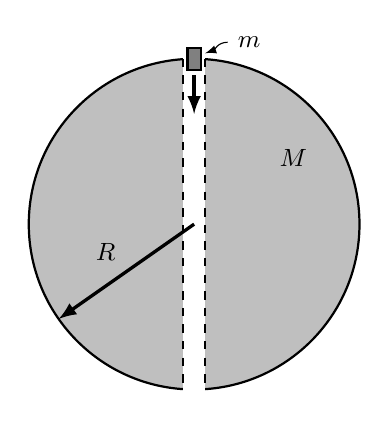
\begin{tikzpicture}[scale=.7,thick]
      \draw[fill=gray!50] circle(3);
      \fill[white](-.2,3.1) rectangle(.2,-3.1);
      \draw[dashed] (-.2,3)--(-.2,-3);
      \draw[dashed] ( .2,3)--( .2,-3);
      \draw[very thick,rotate=-55,->] (0,0)--(0,-3)
      node[midway,above left]{\small $R$};
      \draw[fill=gray] (-.12,3.2) rectangle(.12,2.8);
      \draw[very thick,->](0,2.7)--(0,2);
      \node at (1.8,1.2) {\small $M$};
      \node (m) at (1,3.3) {\small $m$};
      \draw[thin,->] (m) to[out=180, in=20] (.2,3.1);
    \end{tikzpicture}
  }
  \question Suppose that a hole is drilled through the centre of Earth to the
  other side along its axis. A small object of mass $m$ is dropped from rest
  into the hole at the surface of Earth, as shown above. If Earth is assumed to
  be a solid sphere of mass $M$ and radius $R$ and friction is assumed to be
  negligible, correct expressions for the kinetic energy of the mass as it
  passes Earth's centre include which of the following ?
  \begin{enumerate}[nosep]
  \item[I.] $\dfrac12MgR$
  \item[II.] $\dfrac12mgR$
  \item[III.] $\dfrac{GMm}{2R}$
  \end{enumerate}  
  \begin{choices}
    \choice I only
    \choice II only
    \choice III only
    \choice I and III only
    \choice II and III only
  \end{choices}
\end{questions}
\end{document}
